% =========================================================================== %

\begin{frame}[t,plain]
\titlepage
\end{frame}

% =========================================================================== %

\begin{frame}{Code Quality}
%
\begin{columns}
\column{.7\linewidth}
\begin{center}
\includegraphics[width=\linewidth]{./gfx/07-xkcd-codeQuality}\\
\end{center}
%
\column{.2\linewidth}
\small
	\emph{\enquote{I honestly didn't think you could even USE emoji in variable names. Or that there were so many different crying ones.}}

	\vspace{6pt}
	\url{https://xkcd.com/1513/}
\end{columns}
%
\end{frame}

% =========================================================================== %

\begin{frame}{Scope For Today}
%
\begin{itemize}
\item Special Attributes
	\begin{itemize}
	\item \inPy{__doc__}
	\item \inPy{__name__}, \inPy{__qualname__} and \inPy{__module__}
	\item \inPy{__dict__}
	\item \inPy{__code__}
	\end{itemize}
\item Annotations
	\begin{itemize}
	\item \inPy{__annotations__}
	\item Code Linters (aka static analysis)
	\item PyCharm IDE Support
	\end{itemize}
\item More Decorators
	\begin{itemize}
	\item \texttt{functools.wraps}
	\item \texttt{dataclasses.dataclass}
	\item \texttt{atexit.register}
	\end{itemize}
\end{itemize}
%
\end{frame}

% =========================================================================== %

\begin{frame}[fragile]{Special Attributes}
%
\begin{itemize}
\item Automatically generated attributes of functions, classes, class instances and modules
\item Define how code objects behave at runtime
\item Like dunder methods (\zB \inPy{__init__}), but not callable
\item Read/Write access at runtime
	\begin{itemize}
	\item Reading these attributes can make code more concise or enables you to do cool tricks
	\item (Explicitly) writing these attributes leads to the dark side
	\end{itemize}
\end{itemize}
%
\vspace{6pt}
\begin{warnbox}[I won't fix your code ...]
... if you don't heed my warnings. Neither will anybody else.
\end{warnbox}
%
\end{frame}

% =========================================================================== %

\begin{frame}[fragile]{Docstrings -- \inPy{__doc__}}
%
\begin{itemize}
\item Contain's online help-text for any object
	\begin{itemize}
	\item Type \inPy{help(some_object)} in the REPL$^{*)}$ to see the text
	\item Or access it via \inPy{some_object.__doc__} 
	\end{itemize}
\item Actually safe to write that property ...
	\begin{itemize}
	\item E.\;g. \inPy{some_object.__doc__ = "My help on the object"}
	\end{itemize}
\item ... but there's a better way to do so:
	\begin{itemize}
	\item Triple Quoted Strings (\inPy{"""foo bar"""}): May contain line breaks
	\item Automatically used as docstring for the current function, class or module if not assigned to another variable
	\end{itemize}
\end{itemize}
%
\begin{hintbox}[REPL]
$^{*)}$ REPL means \emph{Read-Eval-Print-Loop}, \ie a programming interface where typed lines are executed (evaluated) immediately, like the Python console.
\end{hintbox}
%
\end{frame}

% =========================================================================== %

\begin{frame}[fragile]
%
\begin{codebox}[Example: Function DocString]
\begin{minted}[linenos, fontsize=\scriptsize]{python3}
def print_head(text, width = 80) :
    """
    Prints a boxed headline.
    :param text: the text to put in the box
    :param width: the width in characters of the headline
    :returns: None
    
    Example:
    >>> print_head('headline', 40)
    ########################################
    #               headline               #
    ########################################
    """
    
    formattext = "{" + f":^{width - 4}" + "}"            # e.g. "{:^36}"
    print("#" * width)
    print("# " + formattext.format(text) + " #")
    print("#" * width)

help(print_head)
\end{minted}
\end{codebox}
%
\end{frame}

% =========================================================================== %

\begin{frame}[fragile]
%
\begin{tcbraster}[raster columns=2,
                  raster equal height,
                  nobeforeafter,
                  raster column skip=0.5cm]
\begin{codebox}[Example: Class DocString]
\begin{minted}[fontsize=\scriptsize, linenos]{python3}
class Master :
    """ A masterfully created
        piece of code! """
    
    def __init__(self) :
        """ instantiates a new
            piece of baffling
            awesome software """
        print("master created")
    
    ...
\end{minted}
\end{codebox}
%
\begin{cmdbox}[Output: \texttt{help(Master)}]
\begin{minted}[fontsize=\scriptsize]{text}
class Master(builtins.object)
 |  A masterfully created piece of code!
 |  
 |  Methods defined here:
 |  
 |  __init__(self)
 |      instantiates a new piece of
 |      baffling awesome software
 |  
 |  --------------------------------------
 |  Data descriptors defined here:
 |  
 |  __dict__
 |      dictionary for instance variables
 |     (if defined)
 |  
 |  __weakref__
 |      list of weak references to the
 |      object (if defined)
\end{minted}
\end{cmdbox}
\end{tcbraster}
%
\end{frame}

% =========================================================================== %

\begin{frame}[fragile]
%
\begin{codebox}[Example: Module DocString: TextTools.py]
\begin{minted}[linenos, fontsize=\scriptsize]{python3}
""" 
Text Tools

This module offers helper tools for putting nice text on terminal outputs
"""

def print_head(text, width = 80):
    ...

def print_decobar(width = 80):
    ...
\end{minted}
\end{codebox}
%
\begin{codebox}[Example: Module Docstring: main.py]
\begin{minted}[linenos, fontsize=\scriptsize]{python3}
import TextTools

help(TextTools)
\end{minted}
\end{codebox}
%
\end{frame}

% =========================================================================== %

\begin{frame}{How Is This Better Than Comments?}
%
\begin{columns}[T]
\column{.3\linewidth}
\begin{itemize}
\item Available \enquote{on demand} (without browsing the source)
	\begin{itemize}
	\item Just type \inPy{help(some_class)} in the REPL
	\end{itemize}
\item Inherited by instances
	\begin{itemize}
	\item Typing \inPy{help(my_list)} shows help text for \inPy{class list}
	\end{itemize}
\end{itemize}
%
\column{.3\linewidth}
\begin{itemize}
\item Often IDE-Support
	\begin{itemize}
	\item Hover over function calls to see docstrings
	\item Details vary, but concept widely supported
	\end{itemize}
\end{itemize}
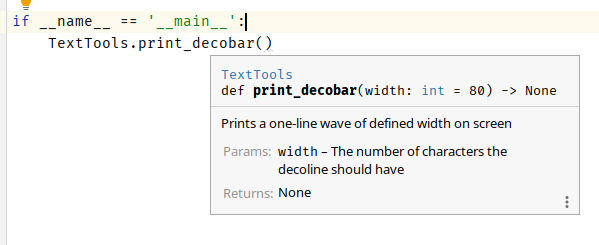
\includegraphics[width=\linewidth]{./gfx/07-helptext-mouseover}
%
\column{.3\linewidth}
\begin{itemize}
\item Two methods for inserting comments allow classification
	\begin{itemize}
	\item \enquote{Normal} comments (\texttt{\#}): explain how code \emph{works}
	\item[\Thus] Needed when you want to \emph{edit} the code
	\item Docstrings: explain how code \emph{is used}
	\item[\Thus] Needed when you want to \emph{use} the code
	\end{itemize}
\end{itemize}
\end{columns}
%
\end{frame}

% =========================================================================== %

\begin{frame}[fragile]
%
\begin{codebox}[Example: DocStrings and Comments]
\begin{minted}[linenos, fontsize=\scriptsize]{python3}
import numpy as np
def numpy_isqrt(number):
    """ approximates 1 / sqrt(number) FAST """
    
    # source: https://github.com/ajcr/ajcr.github.io/blob/
    #              master/_posts/2016-04-01-fast-inverse-square-root-python.md
    # details: https://en.wikipedia.org/wiki/Fast_inverse_square_root#Algorithm
    
    y = np.float32(number)                        # ensure y is a single precision float    
    i = y.view(np.int32)                          # typecast float -> int
    i = np.int32(0x5f3759df) - np.int32(i >> 1)   # evil bit magic, making use of:
                                                  #   log_2(1/sqrt(x)) = -1/2 log_2(x)
    y = i.view(np.float32)                        # typecast int -> float
    
    # one iteration of Newton's method to increase accuracy
    threehalfs = 1.5
    x2 = number * 0.5
    y = y * (threehalfs - (x2 * y * y))
    return float(y)
\end{minted}
\end{codebox}
%
\end{frame}

% =========================================================================== %

\begin{frame}[fragile]{Object Names: \inPy{__name__}, \inPy{__qualname__} and \inPy{__module__}}
%
\begin{itemize}
\item Attribute of functions and classes
	\begin{itemize}
	\item Return name, qualified name and origin module
	\item Name: the name of the function/class
	\item Qualified name: name together with scope in case of nested functions
	\item Module: the name of the module (usually the .py file) in which the function/class is defined
	\item May be useful when functions accept other functions or classes as parameters
	\item E.\;g. \inPy{def tell_and_call(f): print("calling", f.__name__); f()}
	\end{itemize}
\item \inPy{__name__} as non-attribute variable
	\begin{itemize}
	\item Gives either the name of the current module ...
	\item Or \inPy{"__main__"} if in the main module
	\item \texttt{python3 foobar.py}: Any code in \texttt{foobar.py} will identify as \inPy{"__main__"}, other .py files have their \enquote{proper name}
	\item Prevents executing code on \inPy{import}
	\end{itemize}
\end{itemize}
%
\end{frame}

% =========================================================================== %

\begin{frame}[fragile]
%
\begin{codebox}[Example: name variable: LoggerTools.py]
\begin{minted}[linenos, fontsize=\scriptsize]{python3}
""" 
Logger Tools

Facilitates logging events to disk
"""

def log(text):
   print(text, file=logfile)

logfile = open("logfile.txt", "w")       # happens no matter what

if __name__ == "__main__":               # happens only when this
    test_module()                        #  is the main module.
\end{minted}
\end{codebox}
%
\begin{codebox}[Example: Module Docstring: main.py]
\begin{minted}[linenos, fontsize=\scriptsize]{python3}
import LoggerTools

LoggerTools.log("This goes to file")
\end{minted}
\end{codebox}
%
\end{frame}

% =========================================================================== %

\begin{frame}[fragile]{Inner Structure of Composite Objects -- \inPy{__dict__}}
%
\begin{itemize}
\item Internal structure: number and names of attributes
	\begin{itemize}
	\item Can be altered at runtime
	\item Example:
		\begin{itemize}
		\item \texttt{class Foo} defines single attribute \texttt{bar} in its \inPy{__init__}
		\item Instance \texttt{foo = Foo()}
		\item We can add the attribute \texttt{baz} simply by typing \texttt{foo.baz = "something"}
		\item (Does not affect structure of other instances of \texttt{Foo})
		\end{itemize}
	\item Exception: built-in types
		\begin{itemize}
		\item \inPy{int}, \inPy{float}, \inPy{str}, \inPy{list}, \inPy{bytes}, ...
		\end{itemize}
	\end{itemize}
\item Attribute \inPy{__dict__} gives a \inPy{dict} name \thus value of all attributes \enquote{within} the object
	\begin{itemize}
	\item Instance attributes, but not class attributes
	\item Also applies to modules
		\begin{itemize}
		\item Objects in modules are classes and global variables
		\end{itemize}
	\end{itemize}
\item Commands \inPy{vars} and \inPy{dir} (usually) analyze the \inPy{__dict__} attribute
\end{itemize}
%
\end{frame}

% =========================================================================== %

\begin{frame}[fragile]
%
\begin{codebox}[Example: Instance attributes]
\begin{minted}[fontsize=\scriptsize, linenos]{python3}
class Aggregate:
    instance_counter = 0

    def __init__(self):
        Aggregate.instance_counter += 1
        self.content = "some data"

instance = Aggregate()

print("Inspecting instance directly after creation:")
print("  via __dict__:", instance.__dict__)
print("  via vars    :", vars(instance))
\end{minted}
\end{codebox}
%
\begin{cmdbox}[Output:Instance attributes]
\begin{minted}[fontsize=\scriptsize]{text}
Inspecting instance directly after creation:
  via __dict__: {'content': 'some data'}
  via vars    : {'content': 'some data'}
\end{minted}
\end{cmdbox}
%
\end{frame}

% =========================================================================== %

\begin{frame}[fragile]
%
\begin{codebox}[Example: Instance attributes (Continued)]
\begin{minted}[fontsize=\scriptsize, linenos, firstnumber=13]{python3}
print("Inspecting the class itself:")
print(" ", vars(Aggregate))
look_for_attribute = "instance_counter"
print("Looking for a specific member in the class attributes... ")
if look_for_attribute in vars(Aggregate) :
    print(f"  Found '{look_for_attribute}' with value",
          vars(Aggregate)[look_for_attribute])
else:
    print(f"  Attribute '{look_for_attribute}' is not in the class attributes.")
\end{minted}
\end{codebox}
%
\begin{cmdbox}[Output:Instance attributes]
\begin{minted}[fontsize=\scriptsize]{text}
Inspecting the class itself:
  {'__module__': 'ClassInnerStructure', 'instance_counter': 1,
   '__init__': <function Aggregate.__init__ at 0x7f9077170430>, 
   '__dict__': <attribute '__dict__' of 'Aggregate' objects>, 
   '__weakref__': <attribute '__weakref__' of 'Aggregate' objects>, '__doc__': None}
Looking for a specific member in the class attributes... 
  Found 'instance_counter' with value 1
\end{minted}
\end{cmdbox}
%
\end{frame}

% =========================================================================== %

\begin{frame}{Whatsitgudfor?}
%
\begin{itemize}
\item Allows exploiting structure of code to save often tons of tedious coding
\item Example: RPG game
	\begin{itemize}
	\item Characters have properties like \emph{strength}, \emph{charisma}, \emph{intelligence} and \emph{dexterity}
	\item Characters can have a number of items in their backpack that boost these properties
	\item Characters can loose items, too
	\item[\Thus] Task: Compute \emph{current} strength/charisma/...
	\item[\Thus] Naive approach: \inPy{def get_strength(): ...}, \inPy{def get_charisma(): ...}, ...
	\item[\Thus] Better: \inPy{def get_property(property_name): ...}
	\end{itemize}
\end{itemize}
%
\vspace{6pt}
\begin{warnbox}[What it's not good for]
You can also add attributes and even methods at runtime. But that you \emph{can} does not mean that you \emph{should}.
\end{warnbox}
%
\end{frame}

% =========================================================================== %

\begin{frame}[fragile]
%
\begin{codebox}[Example: RPG Game Extract]
\begin{minted}[fontsize=\scriptsize, linenos]{python3}
class Item:
    def __init__(self, name, category, boost):
        self.name = name
        self.category = category
        self.boost = boost

class Person:
    categories = ["strength", "charisma", "intelligence", "dexterity"]
    
    def __init__(self, name):
        self.name = name
        self.backpack = []        
        for category in Person.categories:    # note: don't do this...
            self.__dict__[category] = random.randint(5, 10)

    def get_property(self, category):
        value = self.__dict__[category]
        for item in self.backpack:
            if item.category == category: value += item.boost
        return value
\end{minted}
\end{codebox}
%
\end{frame}

% =========================================================================== %

\begin{frame}[fragile]{Poking Around in the Guts -- \inPy{__code__}}
%
\begin{itemize}
\item Python code is actually \emph{compiled} (\ie translated into \emph{a} machine language)
	\begin{itemize}
	\item Not assembly, not processor directives
	\item But Opcodes of the Python VM
	\end{itemize}
\item Binary data of functions as well as metadata can be accessed after compilation
\item[\Thus] \inPy{__code__} -- returns collection of such metadata
	\begin{itemize}
	\item Has several attributes
	\item \texttt{co\_argcount} -- number of arguments (not including keyword only arguments, * or ** args)
	\item \texttt{co\_code} -- string of raw compiled bytecode
	\item \texttt{co\_filename}, \texttt{co\_firstlineno} -- name of file and number of first line in Python source code in which this code object was created
	\end{itemize}
\item If you really want to go down the rabbit hole
	\begin{itemize}
	\item \url{https://docs.python.org/3/library/inspect.html}
	\item \url{https://docs.python.org/3/library/dis.html}
	\end{itemize}
\end{itemize}
%
\end{frame}

% =========================================================================== %

\begin{frame}[fragile]
%
\begin{codebox}[Example: Arg-Checked Derivative]
\begin{minted}[fontsize=\scriptsize, linenos]{python3}
def derivative(f, epsilon = 1E-6):
    def inner(x):
        return (f(x + epsilon) - f(x - epsilon)) / (2 * epsilon)
    
    if "__call__" in dir(f):   # or: if callable(f)
        if f.__code__.co_args == 1:
            return inner
        else:
            raise AttributeError(f"Function '{f.__name__}' takes " + 
                                  "more than one parameter")
    else:
        raise AttributeError("Not a callable")
\end{minted}
\end{codebox}
%
\begin{cmdbox}[Output: \texttt{derivative.\_\_code\_\_.co\_code}]
\begin{minted}[fontsize=\scriptsize]{text}
b'\x87\x00\x87\x01f\x02d\x01d\x02\x84\x08}\x02d\x03t\x00\x88\x01\x83\x01v\x00r
  \x88\x01j\x01j\x02d\x04k\x02r\x15|\x02S\x00t\x03d\x05\x88\x01j\x04\x9b\x00d
  \x06\x9d\x03d\x07\x17\x00\x83\x01\x82\x01t\x03d\x08\x83\x01\x82\x01'
\end{minted}
\end{cmdbox}
%
\end{frame}

% =========================================================================== %

\begin{frame}{Annotations aka Type Hints}
%
\begin{itemize}
\item Python is \emph{duck typed}
	\begin{itemize}
	\item Data Type of objects can change at runtime
	\item Functions can accept any parameter as long as it's \emph{syntactically compatible}
		\begin{itemize}
		\item \inPy{a + b} will work for \inPy{int}s, \inPy{float}s, \inPy{str}ings, \inPy{list}s, ...
		\item \inPy{(a + b).capitalize()} will only work for \inPy{str}ings
		\end{itemize}
	\end{itemize}
\item Can be cool, often causes trouble
	\begin{itemize}
	\item Accidentally passing wrong data type will crash the program
	\item Not automatically detected; may happen only for specific inputs
	\item[\Thus] Hard to find and remove bugs
	\end{itemize}
\item Type hints: way to tell Python how a function is \emph{intended} to be used
\end{itemize}
%
\begin{hintbox}[Namesake: \emph{Duck Typed Languages} and \emph{Duck Test}]
\footnotesize
\emph{{\color{gray}I can't prove you are a Communist.} But when I see a bird that quacks like a duck, walks like a duck, has feathers and webbed feet and associates with ducks—I'm certainly going to assume that he is a duck.}

\vspace{-18pt}
\begin{flushright}
Emil Mazey, 1946
\end{flushright}
\end{hintbox}
%
\end{frame}

% =========================================================================== %

\begin{frame}{Annotations: Syntax and What They Do}
%
\begin{itemize}
\item Syntax
	\begin{itemize}
	\item Colon + Data type after any declaration
		\begin{itemize}
		\item E.\;g. \inPy{foo: int = 42}
		\end{itemize}
	\item Return values: arrow (\texttt{->}) + Data type
		\begin{itemize}
		\item E.\;g. \inPy{def foo(bar: int) -> str}
		\end{itemize}
	\item Limiting types of containers possible by syntax \texttt{container\_type[containnee\_type]}
		\begin{itemize}
		\item E.\;g. \inPy{data: list[float]}
		\end{itemize}
	\item Type aliases possible to spare you tedious typing and communicate intent
		\begin{itemize}
		\item \inPy{Vector = list[float]} 
		\item \inPy{def dot_product(v1: Vector, v2: Vector) -> float}
		\end{itemize}
	\item Dedicated module \texttt{typing} for more involved typing logic
		\begin{itemize}
		\item E.\;g.: Either a \inPy{float} or an \inPy{int}: \inPy{typing.Union[float, int]}
		\end{itemize}
	\end{itemize}
\item What They Do
	\begin{itemize}
	\item Nothing$^{*)}$
	\end{itemize}
\end{itemize}
%
\end{frame}

% =========================================================================== %

\begin{frame}[fragile]{$^{*)}$ What They \emph{Actually} Do}
%
Type hints are ignored at runtime, but ...
\begin{itemize}
\item They do end up in another special attribute \inPy{__annotations__}
\item They are often used by IDEs
\item They are used by linters
	\begin{itemize}
	\item Linter: \emph{a tool that analyzes source code to flag programming errors, bugs, stylistic errors, and suspicious constructs} (Wikipedia)
	\item For example: mypy -- Linter for Python, written in Python
	\item Often directly built into IDEs (\zB PyCharm)
	\item We'll see how to use that in a couple of slides
	\end{itemize}
\end{itemize}
%
\begin{hintbox}[Namesake: \emph{Linter}]
\footnotesize
Stephen C. Johnson, a computer scientist at Bell Labs, came up with the termin 1978 while working on the C programming language. The term \enquote{lint} was derived from lint, the name for the tiny bits of fiber and fluff shed by clothing, as the tool should act like the lint trap in a clothes dryer, detecting small errors to great effect.
\end{hintbox}
%
\end{frame}

% =========================================================================== %

\begin{frame}[fragile]
%
\begin{codebox}[Example: Annotated Code]
\begin{minted}[fontsize=\scriptsize, linenos]{python3}
import cmath
import typing

Number = typing.Union[int, float, complex]
Vector = typing.Collection[Number]

def dot_product(a: Vector, b: Vector) -> Number:
    if len(a) != len(b):
        raise AttributeError("Vectors do not have same length!")

    return sum(x * y for x, y, in zip(a, b))

def vector_length(v: Vector) -> Number:
    return cmath.sqrt(dot_product(v, v))

def return_untyped_data():
    return ['1', '2', '3']

print(vector_length.__annotations__)
\end{minted}
\end{codebox}
%
\end{frame}

% =========================================================================== %

\begin{frame}[fragile]
%
\begin{codebox}[Example: Annotated Code (Continued)]
\begin{minted}[fontsize=\scriptsize, linenos, firstnumber=last]{python3}
foo = [1, 2, 3]
print(vector_length(foo))

bar: list['str'] = ['1', '2', '3']
print(vector_length(bar))

print(vector_length(return_untyped_data()))
\end{minted}
\end{codebox}
%
\begin{cmdbox}[Output: Annotated Code]
\begin{minted}[fontsize=\scriptsize]{text}
{'v': typing.Collection[typing.Union[int, float, complex]], 
 'return': typing.Union[int, float, complex]}
(3.7416573867739413+0j)

Traceback (most recent call last):
  File "/home/blue-chameleon/Documents/Py_Sci/projects/07-moremeta/TypeHints.py", 
  line 24, in main
    print(vector_length(bar))
  ...
\end{minted}
\end{cmdbox}
%
\end{frame}

% =========================================================================== %

\begin{frame}[fragile]{How \texttt{mypy} Would Have Warned You}
%
\begin{cmdbox}[Install mypy]
\begin{minted}[fontsize=\scriptsize]{text}
$ python3 -m pip install mypy
\end{minted}
%$
\end{cmdbox}
%
\begin{cmdbox}[Output: Annotated Code]
\begin{minted}[fontsize=\scriptsize]{text}
$ mypy --strict TypeHints.py 
TypeHints.py:16: error: Function is missing a return type annotation  [no-untyped-def]
TypeHints.py:24: error: Argument 1 to "vector_length" has incompatible type "List[str]"; 
    expected "Collection[Union[int, float, complex]]"  [arg-type]
TypeHints.py:26: error: Call to untyped function "return_untyped_data" in typed context
    [no-untyped-call]
Found 3 errors in 1 file (checked 1 source file)
\end{minted}
%$
\end{cmdbox}
%
\end{frame}

% =========================================================================== %

\begin{frame}{How Your IDE Might Have Warned You}
%
\begin{columns}[T]
\column{.5\linewidth}
	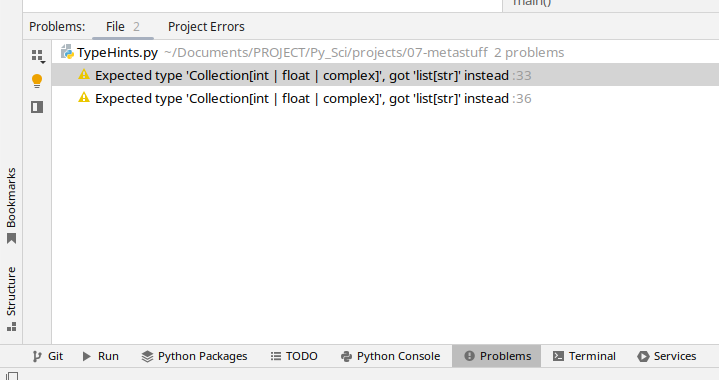
\includegraphics[width=\linewidth]{./gfx/07-pycharm-linter}
%
\column{.4\linewidth}
	\begin{itemize}
	\item Often: Problems Tab
	\item Sometimes: Squiggly lines under code, lightbulbs, etc.
	\item Sometimes: Menu \thus Code/Tools/etc \thus Check/Lint/Analyze/...
	\item Toy around, use the help, or your search engine of choice
		\begin{itemize}
		\item Search for <\emph{name of IDE}> <\emph{linter}>
		\end{itemize}
	\end{itemize}
\end{columns}
%
\end{frame}

% =========================================================================== %

\begin{frame}[fragile]{Decorators and Special Attributes}
%
\begin{itemize}
\item Problem: decorators \enquote{destroy} information in some special attributes
	\begin{itemize}
	\item \inPy{foo.__name__} will give \texttt{foo}, but \inPy{decorator(foo).__name__} will give \texttt{wrapper}
	\item Likewise: \inPy{__qualname__}, \inPy{__module__}, \inPy{__annotations__} and \inPy{__doc__}
	\end{itemize}
\item Solution (manually): copy special attributes from decorated function onto wrapper
\item Solution (simpler): Use \texttt{functools.wraps} decorator on wrapper
%
\begin{codebox}[Schema: Special Attribute Preserving Decorator]
\begin{minted}[fontsize=\scriptsize, linenos]{python3}
def decorator(f):
    @functools.wraps
    def wrapper(*args, **kwargs):
        ...
    return wrapper
\end{minted}
\end{codebox}
\end{itemize}
%
\end{frame}

% =========================================================================== %

\begin{frame}{Using Annotations to Auto-Generate Class Methods}
%
\begin{itemize}
\item Problem: A lot of repetitive boilerplate code when creating classes
	\begin{itemize}
	\item \inPy{__init__} usually only copies attributes into member attributes
	\item Comparator Functions (\inPy{__eq__}, \inPy{__lt__}, ...)
	\item \inPy{__repr__} (A variant to \inPy{__str__})
	\end{itemize}
\item Solution
	\begin{itemize}
	\item Use wrapper \texttt{dataclasses.dataclass} (built-in)
	\item Define attributes as annotations
	\item Done!
	\end{itemize}
\item Particularly useful if you later add attributes, as you don't have to edit all the generated fields
\end{itemize}
%
\begin{hintbox}[Synthesized Comparators]
\footnotesize
Act on the defined attributes, in the order they were defined.
\end{hintbox}
%
\end{frame}

% =========================================================================== %

\begin{frame}[fragile]
%
\begin{codebox}[Example: Dataclasses]
\begin{minted}[fontsize=\scriptsize, linenos]{python3}
@dataclasses.dataclass(order=True)
class InventoryItem:
    name: str
    unit_price: float
    quantity_on_hand: int = 0

def main():
    foo = InventoryItem("Foo", 2)
    bar = InventoryItem("Bar", 5)

    print(foo)
    print(foo < bar)
\end{minted}
\end{codebox}
%
\begin{cmdbox}[Output: Annotated Code]
\begin{minted}[fontsize=\scriptsize]{text}
InventoryItem(name='Foo', unit_price=2, quantity_on_hand=0)
False
\end{minted}
\end{cmdbox}
%
\end{frame}

% =========================================================================== %

\begin{frame}{Links to Explore DataClasses}
%
\begin{itemize}
\item Python Docs
	\begin{itemize}
	\item Full glory of all the created fields, attributes to the wrapper, mechanics in the background
	\item Links to concepts we didn't discuss yet
	\item You should get used to working with the docs, anyway
	\item \url{https://docs.python.org/3/library/dataclasses.html}
	\end{itemize}
\item MCoding
	\begin{itemize}
	\item YouTuber, Mathematician, Software Consultant
	\item Many \textasciitilde 10 min videos on Python under the hood
	\item \url{https://www.youtube.com/watch?v=vBH6GRJ1REM} \\
		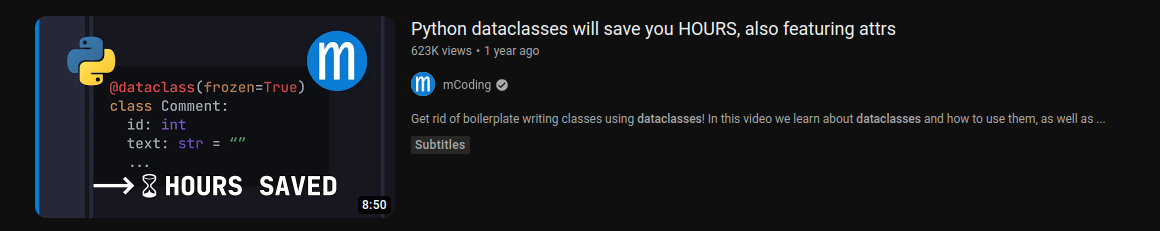
\includegraphics[width=.8\linewidth]{./gfx/07-mcoding-dataclasses}
	\end{itemize}
\end{itemize}
%
\end{frame}

% =========================================================================== %

\begin{frame}{\texttt{atexit}: Automatically Call Functions On Shutdown}
%
\begin{itemize}
\item Assume: Your program needs to do some tidy-up work when it terminates
	\begin{itemize}
	\item E.\;g. closing a file, writing a last log message, turning off a connected machine, ...
	\end{itemize}
\item You could solve that manually ...
	\begin{itemize}
	\item Consider \emph{every possible way} the program could terminate
	\item Menu actions, keyboard shortcuts, end of simulation, ...
	\end{itemize}
\item Or you just register a function
	\begin{itemize}
	\item \texttt{atexit.register(shutdownfunction)}
	\item \texttt{atexit.register(shutdownfunction, arguments, to, the=function)}
	\end{itemize}
\end{itemize}
%
\end{frame}